\documentclass{article}
\usepackage{longtable}
\usepackage{makecell}
\usepackage{float}
\usepackage{booktabs} % 如果要使用更美观的表格线命令,如\toprule等
\usepackage{graphicx}
\usepackage{bm}
\usepackage{gensymb}
\usepackage{placeins}
\usepackage{threeparttable} 
\usepackage{multirow}
\usepackage{aligned-overset}
\usepackage[slantfont,boldfont]{xeCJK}
\usepackage{fontspec}
\renewcommand{\arraystretch}{1.5}
\setCJKmainfont{SimSun}
\setmainfont{SimSun}
\setsansfont{SimSun}

\title{偏振光实验研究实验报告}
\author{2411545 邱凯锐}
\date{2025.4.14}

\begin{document}
\maketitle
\section{实验目的}
\begin{itemize}
    \item 1.理解偏振的基本概念;
    \item 2.熟练掌握马吕斯定律;
    \item 3.掌握线偏振光、椭圆偏振光、圆偏振光的产生方法;
    \item 4.掌握o、e光的区分方法及其偏振关系。
\end{itemize}
\section{实验原理}
\subsection{偏转光的概念}
\hspace*{2em}自由空间中,光是横波,光电场矢量的振动方向应始终与光的传播方向垂直。在垂直于光传播方向的二维平面内,光(电场)矢量的振动状态被称做光波的偏振态。按偏振度划分,光可分为自然光、部分偏振光、完全偏振光。
\begin{itemize}
    \item {自然光:\\可以看成是大量偏振方向不同、彼此无关、无优势振动取向方向的线偏振光的集合。自然光的电场矢量分布相对于传播方向呈轴对称性分布。普通光源(如阳光、烛光、钠灯光等)发的光都是自然光。这是因为光源中所包含的不同原子或分子所发光波,或同一原子不同时刻所发光波,其振动方向、振幅、初始相位各不相同,使得在观测时电场矢量振动在各个方向上的几率相同,没有哪一个方向占更大优势。}
    \item {部分偏振光:\\电场矢量表现出一个占优的振动方向。自然光经过散射、反射或折射一般变成部分偏振光。}
    \item {完全偏振光:\\
    可分为线偏振光、圆偏振光、椭圆偏振光。光电场分布不再杂乱无章,可用解析式表达。}
\end{itemize}
\begin{figure}[ht]
    \centering
    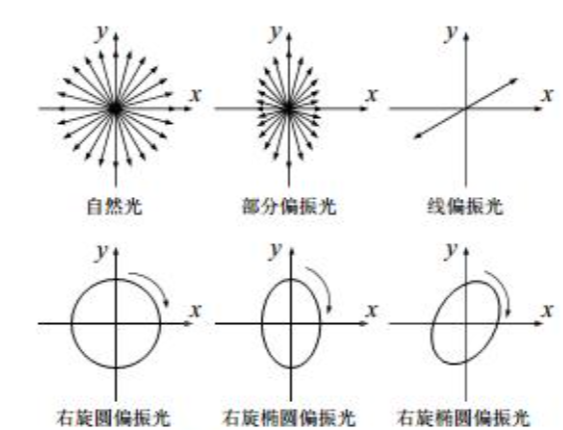
\includegraphics[width=6cm]{1.1.png}
    \caption{光的偏振态}
\end{figure}
\hspace*{2em}\textbf{线偏振光}:\\
\hspace*{2em}在观察时间内,光矢量大小随时间变化,但振动方向始终不变。表达式:
$$
\begin{cases}
E_x(t)=A_x\cos(-\omega t)\\
E_y(t)=A_y\cos(-\omega t + \delta)
\end{cases}
$$
\hspace*{2em}若\(\delta = 0\),偏振于一三象限;若\(\delta = \pi\),偏振于二四象限;偏振极角\(\theta\)取决于振幅比
\[
\tan(\theta)=\frac{A_y}{A_x}\cdot\mathrm{sgn}\{\sin(\delta)\},\theta\in(-\frac{\pi}{2},\frac{\pi}{2}]
\]
\hspace*{2em}\textbf{圆偏振光}:\\
\hspace*{2em}光矢量的大小不变,但方向却随时间改变,沿(逆)着传播方向看矢量端点的轨迹是圆周。可以表达为
\[
\vec{E}(t)=E_x(t)\vec{i} + E_y(t)\vec{j}
\]
或
\[
\begin{cases}
E_x(t)=A\cos(-\omega t)\\
E_y(t)=A\cos\left(-\omega t\pm\frac{\pi}{2}\right)
\end{cases}
\]
\hspace*{2em}其中右旋对应-号,左旋对应+号。\\
\hspace*{2em}\textbf{椭圆偏振光}:\\
\hspace*{2em}和圆偏振光类似,光矢量的大小和方向都随时间改变,矢量端点的轨迹是椭圆。可以表达为
\[
\vec{E}(t)=E_x(t)\vec{i}+E_y(t)\vec{j}
\]
或
\[
\begin{cases}
E_x(t)=A_x\cos(-\omega t+\varphi_x)\\
E_y(t)=A_y\cos\left(-\omega t+\varphi_y\right)
\end{cases}
\]
\hspace*{2em}椭圆偏振态可由极角和椭偏角来描述。
\begin{figure}[ht]
    \centering
    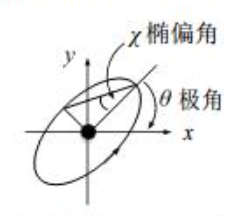
\includegraphics[width=5cm]{1.2.png}
    \caption{椭圆偏振光的极角和椭偏角的定义}
\end{figure}\\
\hspace*{2em}为了描述非偏振光的偏振性的强弱,引入偏振度的概念,设其优势振动方向的光强为\(I_{\max}\),处于最劣势的振动方向光强为\(I_{\min}\),那么偏振度为
\[
P = \frac{I_{\max}-I_{\min}}{I_{\max}+I_{\min}}
\]
\subsection{偏振光的产生}
\hspace*{2em}为了便于在理论上利用电磁学或电动力学进行处理,我们在实验上研究光 - 物质相互作用时,一般使用偏振光,这使得我们必须要掌握偏振光的产生方法:
\begin{itemize}
    \item \textbf{二向色性}:\\
    \hspace*{2em}二向色性原指各向异性的晶体对不同振动方向的偏振光有不同的吸收系数,然而这种性质还与光波的波长有关,进而对于由振动方向相垂直而合成的线偏振白光通过该晶体后会呈现不同的颜色,故称二向色性。\\
    \hspace*{2em}二向色性片的制作方法比较简单,比如将聚乙烯醇薄膜浸泡在碘溶液中,这就形成了碘链,然后在高温环境下将其拉伸形成碘 - 聚乙烯醇构成的长链(它是可以导电的),最后烘干制成。对于入射光,平行于长链振动的分量会对电子做功而被强烈吸收;垂直于长链的分量可以透过,从而得到线偏振光,光矢量垂直于拉伸方向。本实验中所使用的偏振片即为二向色性片。
    \begin{figure}[ht]
        \centering
        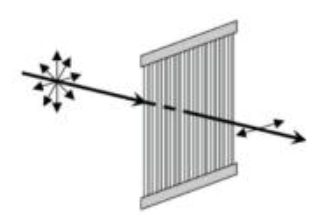
\includegraphics[width=3cm]{2.1.png}
        \caption{二向色性}
    \end{figure}
    \item \textbf{双折射}:\\
    \hspace*{2em}当自然光入射到各向同性介质时,只有一束折射光。而对于各向异性的晶体,则会有两束折射光,称这种现象为双折射(birefringence)。人们发现这两束光都是线偏振光。同时,晶体中存在一个特殊的方向,当光沿这个方向传播时不发生双折射,这个方向称为晶体的光轴(optical axis of crystal)。\\
    \hspace*{2em}在单轴晶体中,两条折射光线的其中一条完全满足折射定律,保持在入射面内传播,这束光称为寻常光线,也称 o 光(ordinary ray);而对于另一束光,从实验上看其传播特性不满足折射定律(思考折射率是否被打破),其入射角的正弦与折射角的正弦之比不是常数,且通常不在入射面内,这束光称为非寻常光线,也称 e 光(extraordinary ray)。\\
    \hspace*{2em}o 光、e 光间的折射率差异为起偏提供了方法,比如图4,两个由双折射晶体制作的直角棱镜,利用树脂胶(折射率 \(n_g\))粘合在一起,保证 \(n_g\) 要略大于并接近 \(n_e\) ,但小于 \(n_o\)(反之亦然),使 \(\theta\) 大于 o 光在斜面界面的临界角,那么 o 光会在界面上发生全反射,而e光由于两介质折射率接近,所以几乎无偏折地从棱镜出射。这也是格兰 - 汤姆逊(Glan - Thompson)棱镜的工作原理(建议查询其他棱镜,如格兰 - 傅科(Glan - Foucault)棱镜、沃拉斯顿(Wollaston)棱镜等的原理)。
    \begin{figure}[ht]
        \centering
        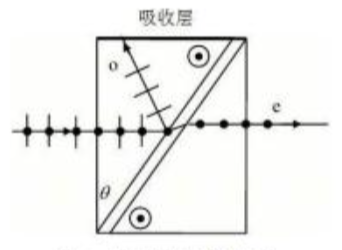
\includegraphics[width=4cm]{2.2.png}
        \caption{双折射起偏原理}
    \end{figure}
    \item \textbf{玻片堆}:\\
    \hspace*{2em}菲涅尔公式告诉我们,对于斜入射,反射光和折射光中的 \(s\) 和 \(p\) 偏振成分的反射系数和透射系数都是不同的,这就意味着反射和折射都会改变光的偏振态。如此我们采用一堆平行放置的玻璃片,在每一层玻璃片上都产生上面所说的现象,经过 \(N\) 层玻璃片之后,折射光线中的 \(s\) 偏振几乎可以认为没有了,只留下 \(p\) 偏振光。
    \begin{figure}[ht]
        \centering
        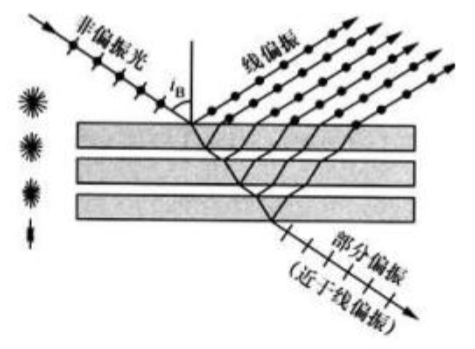
\includegraphics[width=4cm]{2.3.png}
        \caption{拨片堆起偏原理}
    \end{figure}
\end{itemize}
\subsection{偏振态的转化}
\hspace*{2em}利用波片可以由线偏振光产生圆偏光与椭圆偏振光。双折射晶体中 \(o\) 光和 \(e\) 光的折射率不同,且它们的波面是分开的,可以据此制成相位延迟波片。传播速度快的光分量其电场振动方向被称为快轴方向(即负晶体的 \(e\) 轴,正晶体的 \(o\) 轴),反之成为慢轴。
\begin{itemize}
    \item \textbf{半波片}:\\
    \hspace*{2em}快、慢光间产生 \(\pi\) 的相位差,线偏振光通过后仍然为线偏振光,电场矢量的振动方向相对于快(慢)轴对称。
    \begin{figure}[ht]
        \centering
        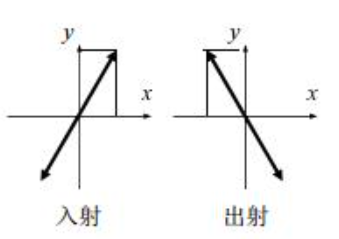
\includegraphics[width=4cm]{3.1.png}
        \caption{半波片工作原理}
    \end{figure}
    \item \textbf{1/4波片}:\\
    \hspace*{2em}经过1/4波片,快、慢光间产生\(\pm\pi/2\)的额外相位差。当入射线偏振方向与光轴夹角为\(\pi/4\)时,出射光为圆偏振光。
    \begin{figure}[ht]
        \centering
        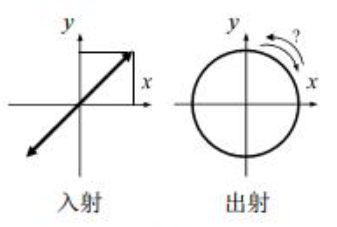
\includegraphics[width=4cm]{3.2.png}
        \caption{1/4波片工作原理}
    \end{figure}
\end{itemize}
对于其他情况,均产生椭圆偏振光。
\subsection{偏振态分析}
\hspace*{2em}光波的电场分量为矢量,也满足矢量分解法则。1808年,马吕斯经实验指出,强度为\(I_0\)的线偏振光,透过检偏片后,透射光的强度(不考虑吸收)为:
\[
I = I_0 (\cos\alpha)^2
\]
\hspace*{2em}其中,\(\alpha\)为入射线偏振光的电场振动方向和检偏器极角方向之间的夹角。该式称为马吕斯定律。
\section{实验仪器}
\begin{itemize}
    \item 半导体激光器(波长为650纳米),光接收器 
    \item 偏振片(2个),半波片,1/4波片,冰洲石晶体
\end{itemize}
\section{实验光路图}
\begin{figure}[ht]
    \centering
    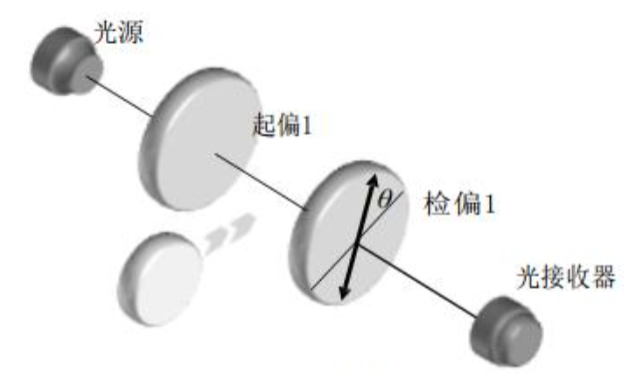
\includegraphics[width=6cm]{4.1.png}
    \caption{试验系统}
\end{figure}
\section{实验步骤}
\subsection{准备系统}
(1)将实验器材如光路图所示顺序摆在旋转位移滑座上,并保证激光照射在接收器上;\\
(2)旋转检偏片一圈,观察接收器上的示数,确认接收器没有饱和或为 0;\\
(3)旋转检偏片,将起偏片与检偏片调为正交。定义此时的检偏片的极角方向为 0 度,并以此建立极坐标系。
\subsection{验证马吕斯定律}
(1)旋转起偏器$\alpha=30\degree$角。旋转检偏片角度$(\theta)$半周(以$5\degree$为步长),并同时记录接收器示数。\\
(2)画$I(\theta)$图,利用马吕斯定律拟合曲线,求得起偏角$\alpha$,同设定值比较,进行误差分析。\\
\hspace*{2em}根据拟合曲线得到$I_1=2.0144\cos^2(0.9818\theta-0.5207)-0.0164$,其中$\theta$转化为弧度制,$\alpha=-0.5207=29.83\degree$。
\begin{figure}[ht]
    \centering
    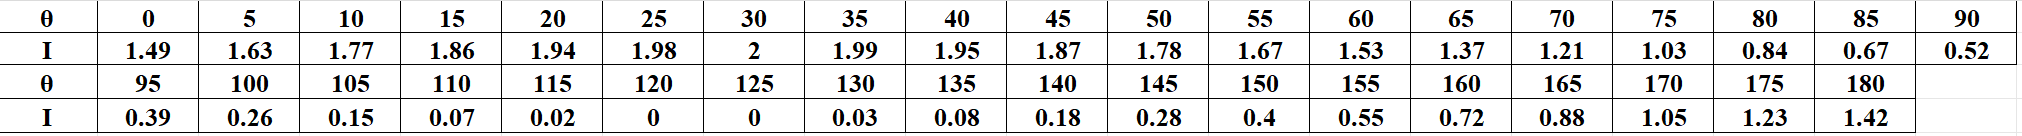
\includegraphics[width=12cm]{5.1.png}
\end{figure}
\begin{figure}[ht]
    \centering
    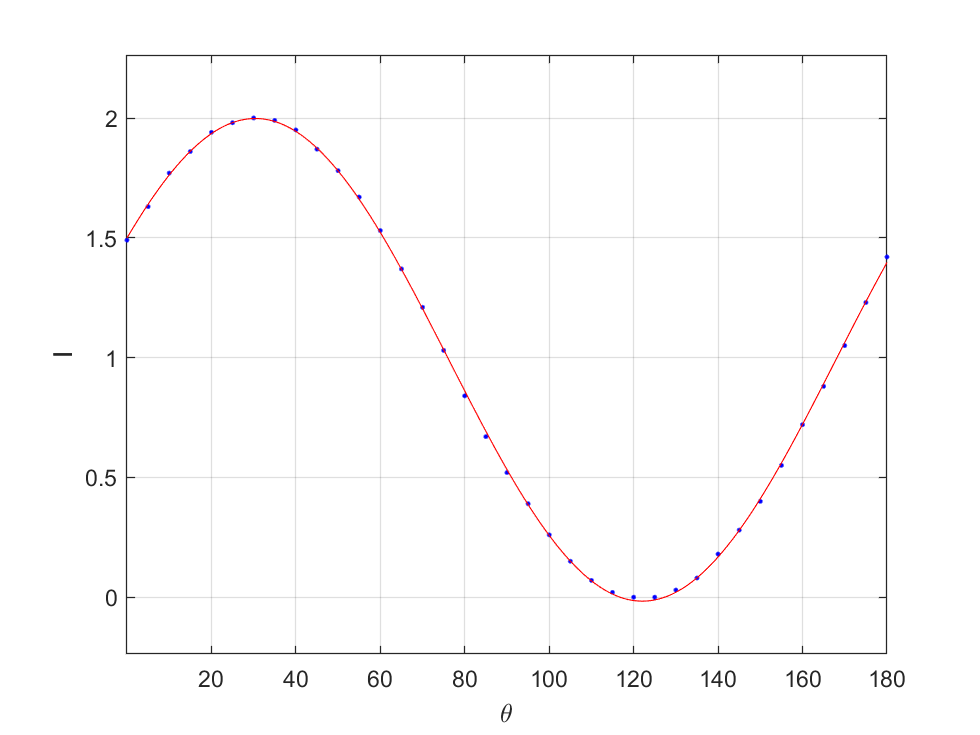
\includegraphics[width=7cm]{1.png}
\end{figure}
\subsection{验证半波片工作原理}
(1)将检偏片恢复 0 点,旋转起偏片,与检偏片正交,在两偏振片之间插入半波片;\\
(2)旋转半波片一圈,观察接收器上的示数,确认接收器没有饱和或为 0;\\
(3)旋转半波片至消光;\\
(4)旋转半波片$\alpha=30\degree$角;\\
(5)旋转检偏片角度$(\theta)$半周(以$5\degree$为步长),并同时记录接收器示;\\
(6)画\(I(\theta)\)图,利用马吕斯定律拟合曲线,求得此时的偏振极角,验证半波片作用,并进行误差分析。\\
\hspace*{2em}根据拟合曲线得到$I_1=1.3740\cos^2(0.9783\theta-0.4734)-0.0125$,其中$\theta$转化为弧度制,$\alpha=-0.4734=27.12\degree$。
\begin{figure}[ht]
    \centering
    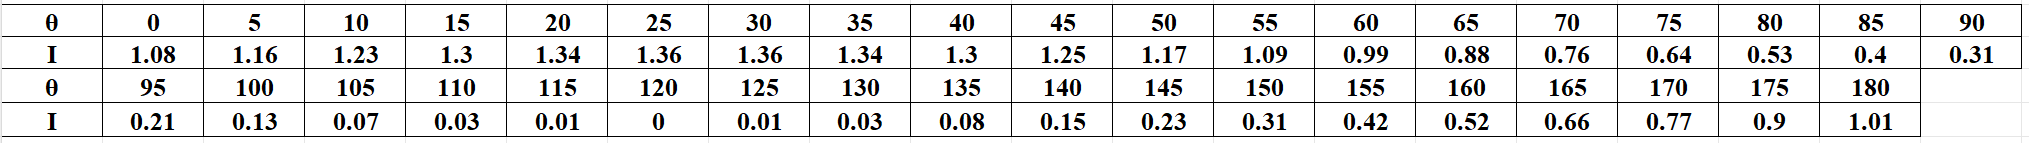
\includegraphics[width=12cm]{5.2.png}
\end{figure}
\begin{figure}[!h]
    \centering
    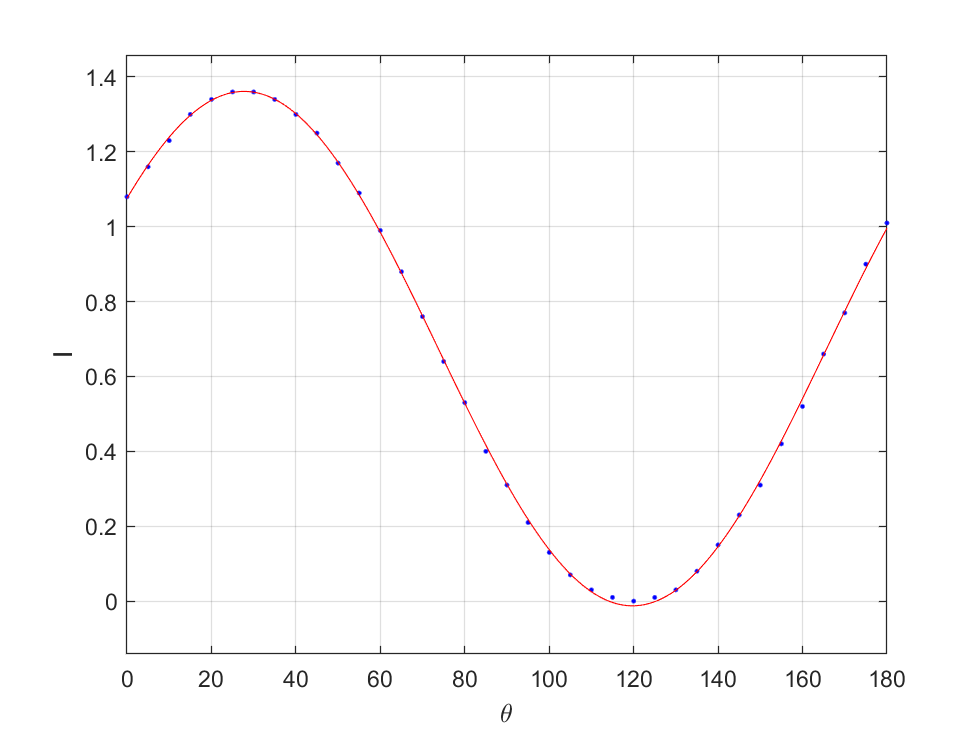
\includegraphics[width=7cm]{2.png}
\end{figure}
\subsection{验证1/4波片工作原理}
(1)将检偏片恢复0点,旋转起偏片,与检偏片正交,在两偏振片之间插入1/4波片;\\
(2)旋转1/4波片一圈,观察接收器上的示数,确认接收器没有饱和或为0;\\
(3)旋转1/4波片至消光;\\
(4)旋转1/4波片$\alpha$角$(\alpha\neq 45\degree)$;\\
(5)旋转检偏片角度$(\theta)$半周(以$5\degree$为步长),并同时记录接收器示数;\\
(6)画\(I(\theta)\)图,利用马吕斯定律拟合曲线,验证出射光是否椭圆偏振光,并进行误差分析,计算极角与椭偏角。\\
\hspace*{2em}图象没有零点,结合极图可以判断为椭圆偏振光,极角为$0\degree$,椭偏角为$38.29\degree$
\begin{figure}[ht]
    \centering
    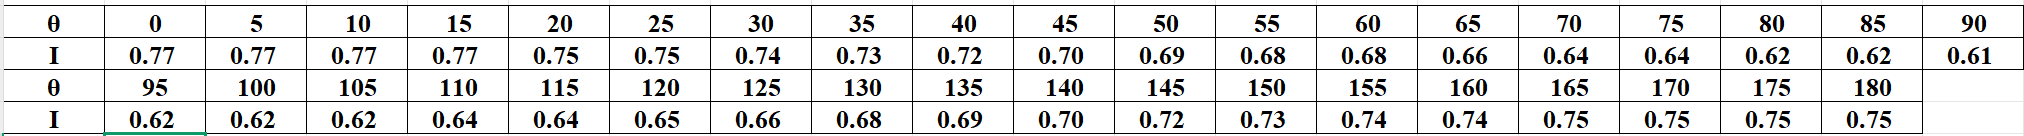
\includegraphics[width=12cm]{5.3.png}
\end{figure}
\begin{figure}[!h]
    \centering
    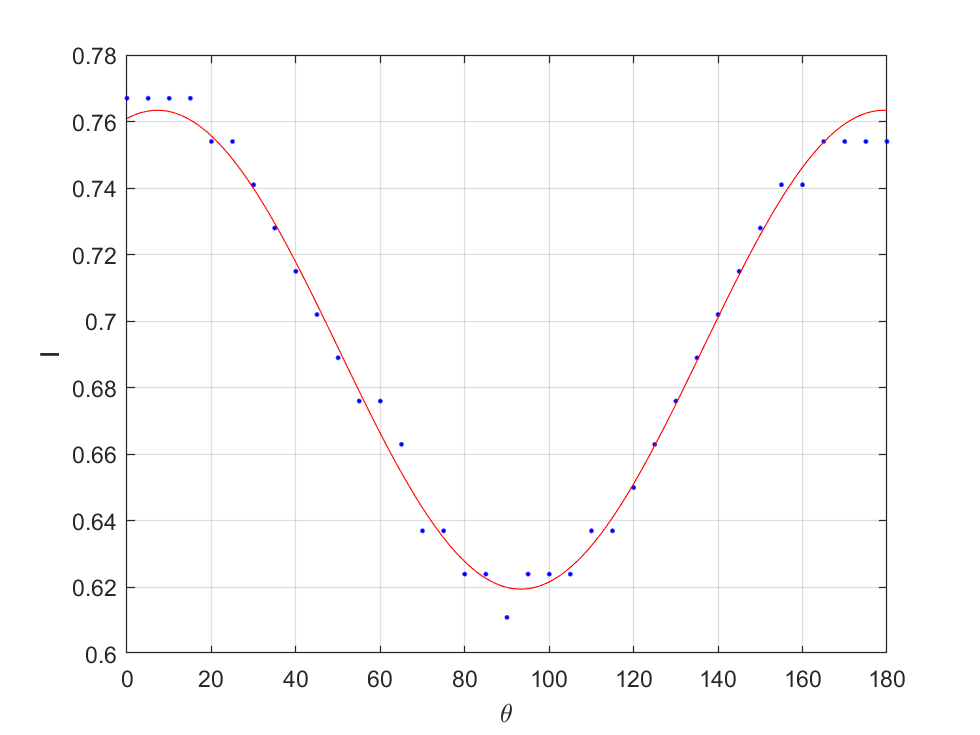
\includegraphics[width=7cm]{3.png}
\end{figure}
\begin{figure}[!h]
    \centering
    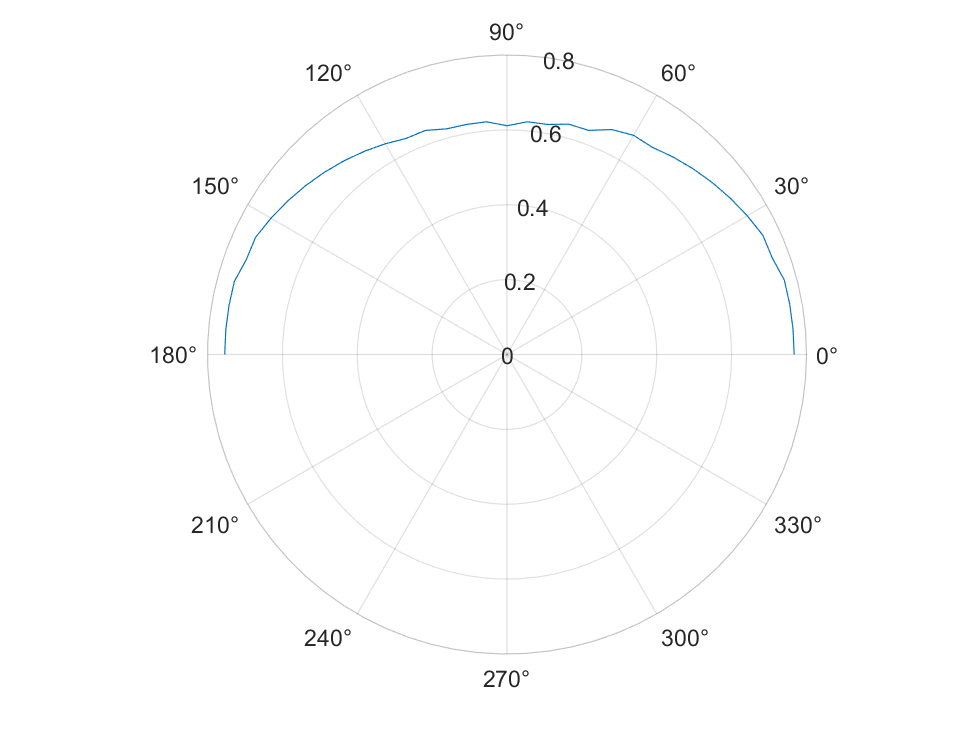
\includegraphics[width=7cm]{33.png}
\end{figure}
\subsection{圆偏振光产生}
(1)旋转1/4波片至消光;\\
(2)旋转1/4波片$45\degree$;\\
(3)旋转检偏片角度(\(\theta\))半周(以$5\degree$为步长并同时记录接收器示数;\\
(4)画\(I(\theta)\)图,利用马吕斯定律拟合曲线,验证出射光是否圆偏振光,并进行误差分析。\\
\hspace*{2em}图象没有0点,由于波片、光源以及接收器存在一定的系统误差,结合极图后半段较为接近圆形,大致判断为圆偏振光。
\begin{figure}[ht]
    \centering
    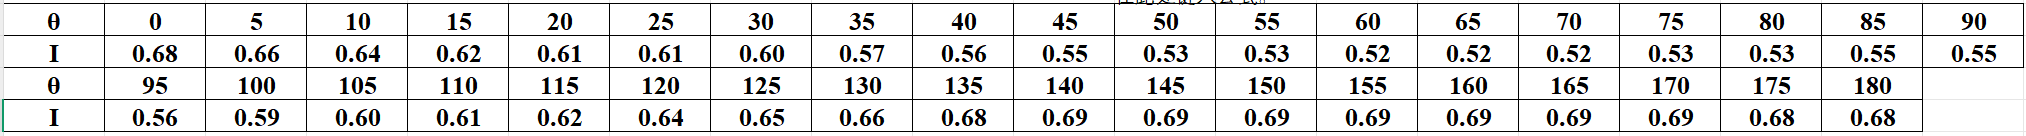
\includegraphics[width=12cm]{5.4.png}
\end{figure}
\begin{figure}[!h]
    \centering
    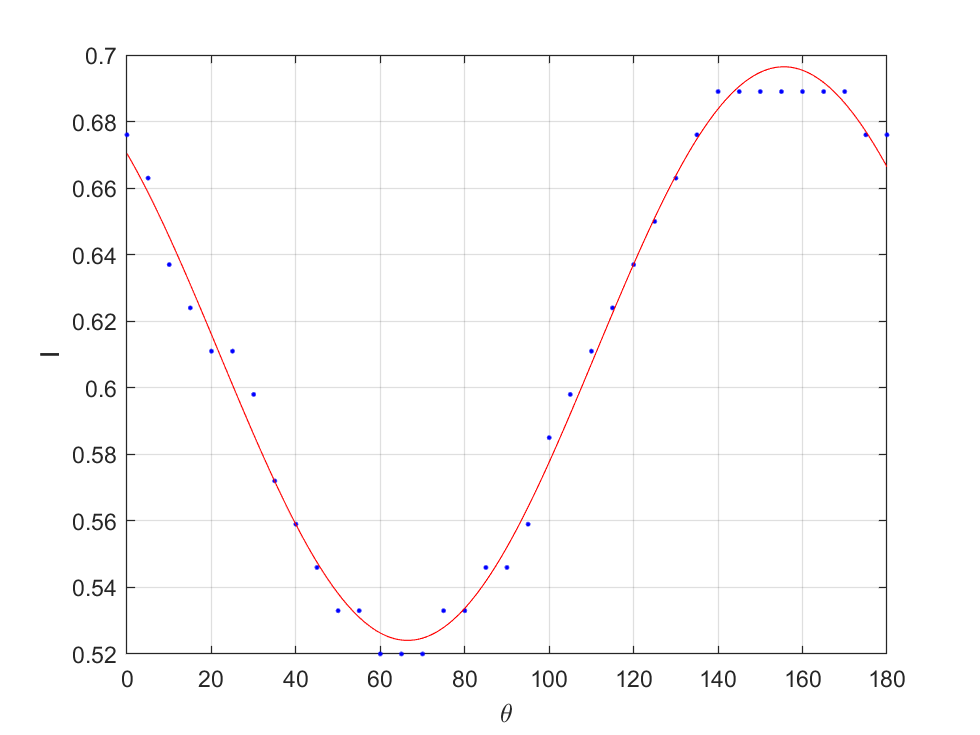
\includegraphics[width=7cm]{4.png}
\end{figure}
\begin{figure}[!h]
    \centering
    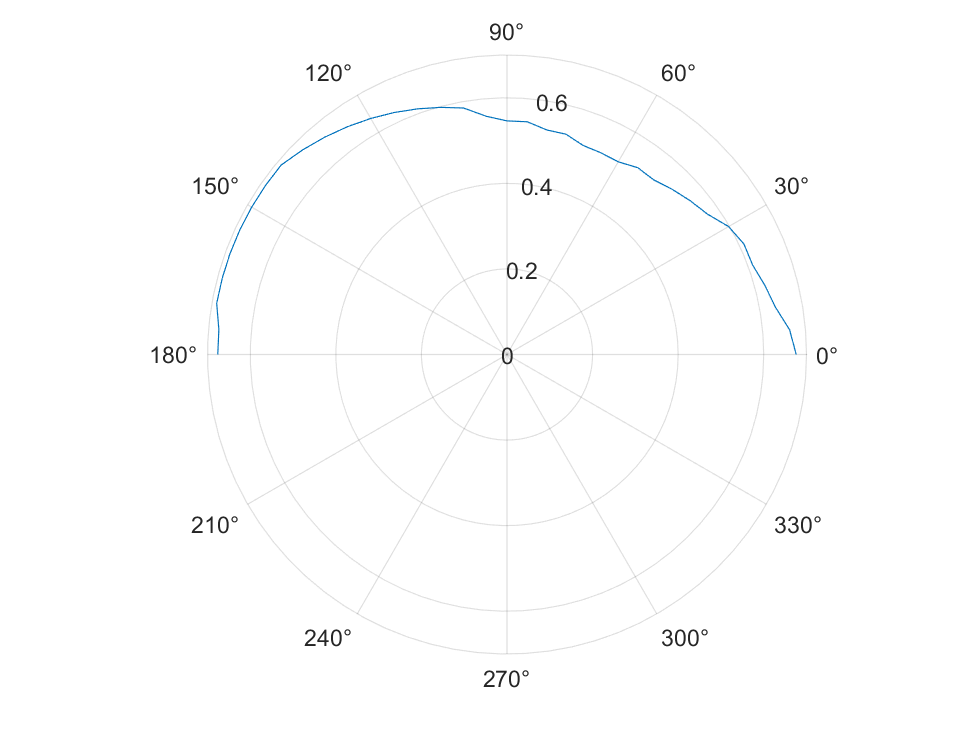
\includegraphics[width=7cm]{44.png}
\end{figure}
\subsection{验证波片堆工作原理}
(1)将检偏片恢复0点;\\
(2)去掉起偏片;\\
(3)插入玻片堆,并调整其位置,使激光打在接收器上;\\
(4)旋转检偏片角度($\theta$)半周(以$5\degree$为步长),并同时记录接收器示数;\\
(5)画$I(\theta)$图,利用马吕斯定律拟合曲线,验证出射光是否为偏振光,是线偏振光、圆偏振光,还是椭圆偏振光?\\
\hspace*{2em}图象存在0点,且符合马吕斯定律,可以判断为线偏振光。
\begin{figure}[ht]
    \centering
    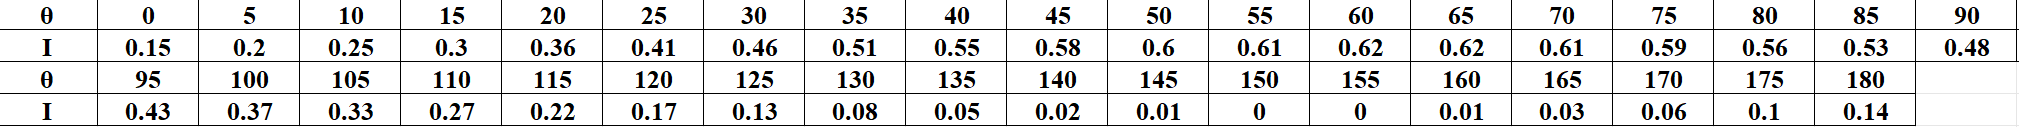
\includegraphics[width=12cm]{5.5.png}
\end{figure}
\begin{figure}[ht]
    \centering
    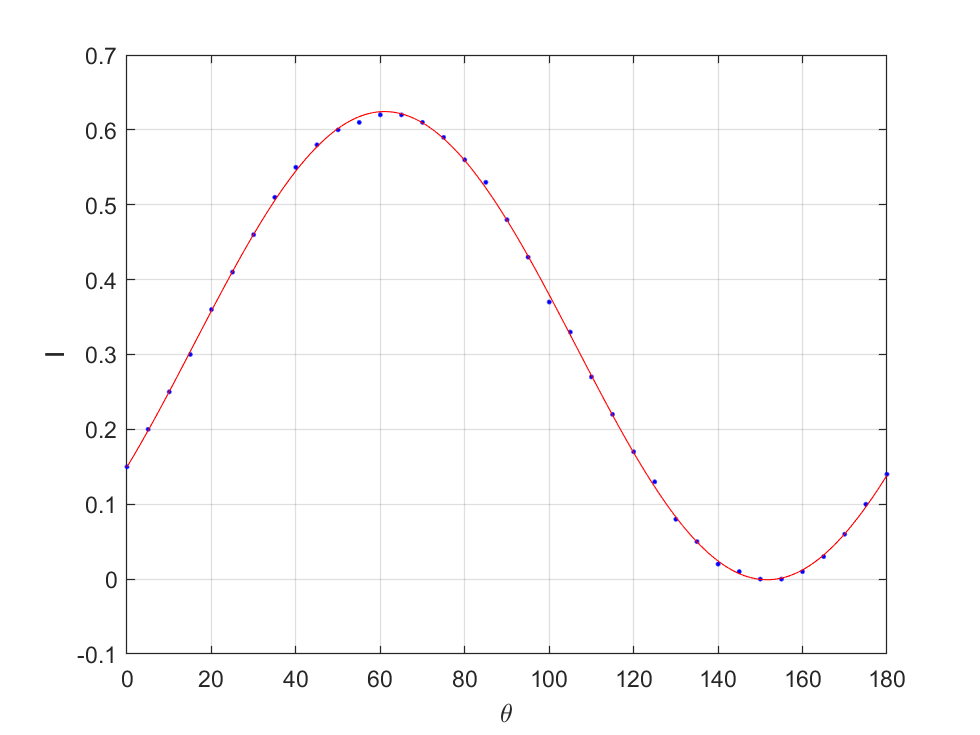
\includegraphics[width=7cm]{5.png}
\end{figure}
\subsection{双折射晶体o,e光的判断}
(1)将检偏片恢复0点\\
(2)去掉起偏片;\\
(3)插入双折射晶体(从小孔方向入射),并调整其位置,在后方使用光屏观察透射光。\\
(4)对两个光斑,判断o, e光;
\begin{figure}[ht]
    \centering
    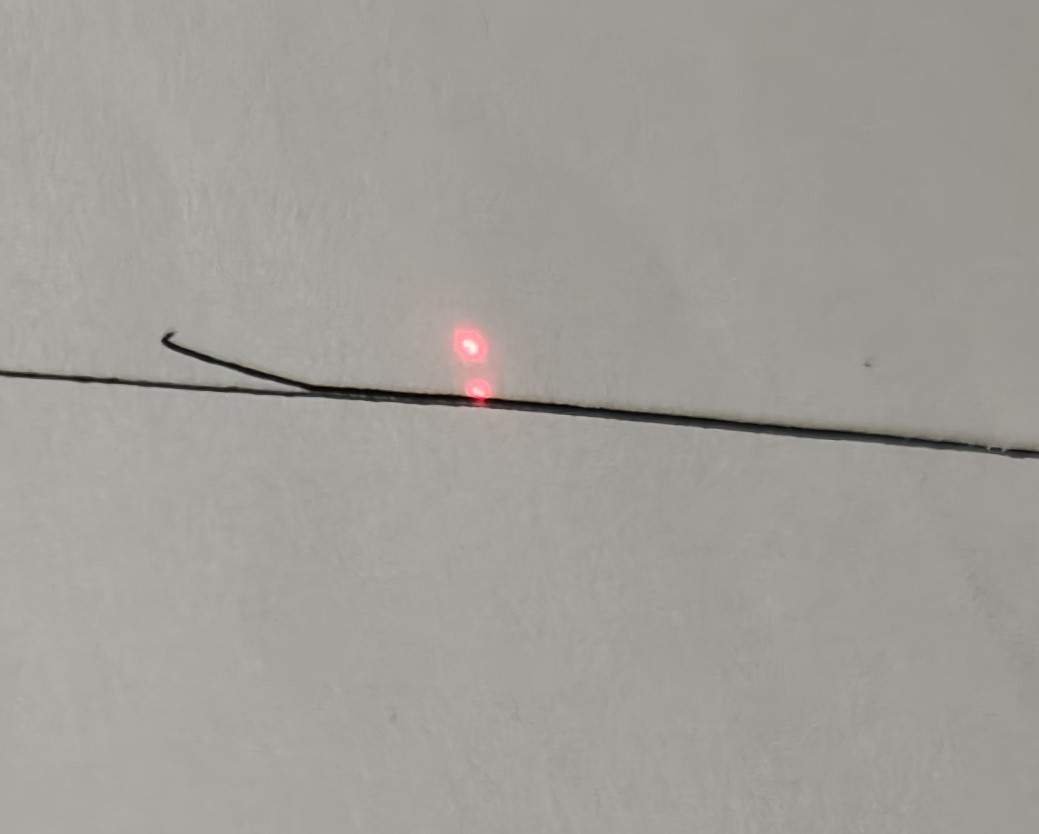
\includegraphics[width=7cm]{6.jpg}
\end{figure}\\
\hspace*{2em}观察到有两个光斑,旋转冰洲石,发现一个光斑几乎不发生移动,为e光,另一个光斑作近似圆周运动,为o光。
\section{思考题}
1.\textbf{自然界中最普遍存在的偏振态是哪种?}\\
\hspace*{2em}线偏振光,因为自然界反射、折射等现象产生的主要是线偏振光。\\
2.\textbf{我们是否能使用单个光学元件由自然光产生圆偏振光或椭圆偏振光?}\\
\hspace*{2em}不能,单个光学元件难以同时改变光沿不同方向的振动情况和光的相位,所以无法使自然光转变为圆偏振光和椭圆偏振光。\\
3.\textbf{理论上讲,我们所学习的 1/4 波片产生圆偏振光的方法是否严格?如果不是,什么原因?如何能产生严格的圆偏振光?}\\
\hspace*{2em}理论上讲,利用1/4波片产生圆偏振光的方法使严格成立的。但在实际操作中,受到入射的线偏光,波片精度等影响,难以产生严格的圆偏光。
对此,为了产生严格的圆偏光,我们应该确保入射光为严格的线偏光,确保入射的方向和角度足够精确,1/4波片精度足够高。同时可以实时监控产生的偏振光,不断校准系统,产生较为严格的圆偏光。
\end{document}